\section{Awareness: The Decision Filter}
\label{sec:awareness}

%%%%%%%%%%%%%%%%%%%%%%%%%%%%%%%%%%%%%%%%%%%%%%%%%%%%%%%%%%%%%%%%%%%%%%%%%%%%%%%
% CHAPTER 11: The Awareness Function (AWA) - REVISED
% Correct definition: Consciousness of effects on utility levels
%%%%%%%%%%%%%%%%%%%%%%%%%%%%%%%%%%%%%%%%%%%%%%%%%%%%%%%%%%%%%%%%%%%%%%%%%%%%%%%

Chapter~\ref{sec:fepsde-utility} established what \emph{could} generate utility:
144 components across three categories (INU, KNU, IDN), six dimensions (FEPSDE),
four time horizons, and two valences. But this full welfare structure exists
only in theory. In any actual decision moment, people are not aware of all
potential effects their behavior has.

This chapter introduces the \textbf{Awareness Function}: the consciousness
that filters which utility effects are perceived at the moment of decision.

%%%%%%%%%%%%%%%%%%%%%%%%%%%%%%%%%%%%%%%%%%%%%%%%%%%%%%%%%%%%%%%%%%%%%%%%%%%%%%%
\subsection{Definition: What Is Awareness?}
\label{subsec:awareness-definition}
%%%%%%%%%%%%%%%%%%%%%%%%%%%%%%%%%%%%%%%%%%%%%%%%%%%%%%%%%%%%%%%%%%%%%%%%%%%%%%%

\subsubsection{The Formal Definition}

\begin{definition}[Awareness]
\label{def:awareness}
\textbf{Awareness} is the consciousness of the positive and negative effects 
on one's own utility level (INU, KNU, IDN) and on the utility level (INU, KNU, IDN) 
of a relevant community, that a person has at the moment of decision or 
exhibited behavior.
\end{definition}

\paragraph{In German:}
\textit{Awareness ist das Bewusstsein über die positiven und negativen Effekte 
für das eigene Nutzenlevel (INU, KNU, IDN) und das Nutzenlevel (INU, KNU, IDN) 
einer relevanten Community, die ein Mensch im Moment der Entscheidung / 
des gezeigten Verhaltens hat.}

\subsubsection{Analytical Decomposition of the Definition}

The definition contains seven distinct elements. Each requires precise understanding:

\begin{table}[htbp]
\centering
\caption{Seven Elements of the Awareness Definition}
\label{tab:awareness-elements}
\renewcommand{\arraystretch}{1.4}
\begin{tabular}{@{}clp{7cm}@{}}
\toprule
\textbf{\#} & \textbf{Element} & \textbf{Meaning} \\
\midrule
1 & Consciousness & Active mental representation, not just potential \\
2 & Positive and negative effects & Both Gains and Pains, not just one \\
3 & Utility level & The 144-component structure from Chapter 10 \\
4 & Own (INU, KNU, IDN) & All three categories for the self \\
5 & Relevant community & Specific others whose welfare matters \\
6 & Community's (INU, KNU, IDN) & All three categories for others \\
7 & Moment of decision/behavior & Situational, not abstract \\
\bottomrule
\end{tabular}
\end{table}

%%%%%%%%%%%%%%%%%%%%%%%%%%%%%%%%%%%%%%%%%%%%%%%%%%%%%%%%%%%%%%%%%%%%%%%%%%%%%%%
\subsection{Element 1: Consciousness}
\label{subsec:consciousness}
%%%%%%%%%%%%%%%%%%%%%%%%%%%%%%%%%%%%%%%%%%%%%%%%%%%%%%%%%%%%%%%%%%%%%%%%%%%%%%%

\paragraph{What Consciousness Means Here.}
Awareness requires \emph{active mental representation}---the person must 
actually be thinking about the effects, not merely having the theoretical 
capacity to think about them.

\begin{table}[htbp]
\centering
\caption{Consciousness vs. Potential Knowledge}
\label{tab:consciousness-vs-potential}
\renewcommand{\arraystretch}{1.3}
\begin{tabular}{@{}lll@{}}
\toprule
\textbf{State} & \textbf{Description} & \textbf{Behavioral Impact} \\
\midrule
No knowledge & Person doesn't know the effect exists & None \\
Latent knowledge & Knows but not thinking about it & None \\
\textbf{Conscious awareness} & \textbf{Actively thinking about it} & \textbf{Guides behavior} \\
\bottomrule
\end{tabular}
\end{table}

\paragraph{The Knowledge-Awareness Gap.}
A person may \emph{know} that smoking causes cancer ($U^{INU}_{P,3}$ effect)
but not be \emph{conscious} of this at the moment of lighting a cigarette.
Knowledge is necessary but not sufficient for awareness.

\begin{equation}
\text{Knowledge} \not\Rightarrow \text{Awareness}
\end{equation}

\paragraph{Degrees of Consciousness.}
Consciousness is not binary but graded:

\begin{equation}
a \in [0, 1]
\end{equation}

\begin{itemize}
\item $a = 0$: Not conscious at all (effect not in working memory)
\item $a = 0.3$: Dimly aware (peripheral, not focal)
\item $a = 0.7$: Clearly aware (actively considering)
\item $a = 1$: Fully conscious (central to decision)
\end{itemize}

%%%%%%%%%%%%%%%%%%%%%%%%%%%%%%%%%%%%%%%%%%%%%%%%%%%%%%%%%%%%%%%%%%%%%%%%%%%%%%%
\subsection{Element 2: Positive and Negative Effects}
\label{subsec:positive-negative}
%%%%%%%%%%%%%%%%%%%%%%%%%%%%%%%%%%%%%%%%%%%%%%%%%%%%%%%%%%%%%%%%%%%%%%%%%%%%%%%

\paragraph{Both Directions Matter.}
Awareness encompasses consciousness of \emph{both}:
\begin{itemize}
\item \textbf{Positive effects}: Gains ($G$) from the action
\item \textbf{Negative effects}: Pains ($P$) from the action
\end{itemize}

\paragraph{Asymmetric Awareness.}
People often have asymmetric awareness of positive vs. negative effects:

\begin{table}[htbp]
\centering
\caption{Asymmetric Awareness Patterns}
\label{tab:asymmetric-awareness}
\renewcommand{\arraystretch}{1.3}
\begin{tabular}{@{}lll@{}}
\toprule
\textbf{Pattern} & \textbf{Description} & \textbf{Example} \\
\midrule
Gain-focused & High $a_G$, low $a_P$ & Excited buyer ignores costs \\
Pain-focused & Low $a_G$, high $a_P$ & Anxious person sees only risks \\
Balanced & $a_G \approx a_P$ & Deliberate decision-making \\
\bottomrule
\end{tabular}
\end{table}

\paragraph{The Awareness Vector (Extended).}
For complete specification, awareness has both a category dimension and 
a valence dimension:

\begin{equation}
a^i_v \quad \text{where } i \in \{INU, KNU, IDN\}, \; v \in \{G, P\}
\end{equation}

This yields 6 awareness parameters for own utility, and 6 more for 
community utility (see below).

%%%%%%%%%%%%%%%%%%%%%%%%%%%%%%%%%%%%%%%%%%%%%%%%%%%%%%%%%%%%%%%%%%%%%%%%%%%%%%%
\subsection{Element 3: Utility Level}
\label{subsec:utility-level}
%%%%%%%%%%%%%%%%%%%%%%%%%%%%%%%%%%%%%%%%%%%%%%%%%%%%%%%%%%%%%%%%%%%%%%%%%%%%%%%

\paragraph{Connection to Chapter 10.}
``Utility level'' refers to the complete 144-component structure:

\begin{equation}
U = \{U^i_{d,t}\} \quad \text{for } i \in \{INU, KNU, IDN\}, \; d \in FEPSDE, \; t \in \{0,1,2,3\}
\end{equation}

\paragraph{Awareness as Utility Filter.}
Awareness determines which of these 144 components enter the decision:

\begin{equation}
U^{eff} = \sum_{i,d,t} a^i_{d,t} \cdot U^i_{d,t}
\end{equation}

In practice, we use the simplified category-level form:

\begin{equation}
U^{eff}_i = a_i \cdot U^i
\end{equation}

\paragraph{What ``Effects on Utility Level'' Means.}
When we say awareness of ``effects on utility level,'' we mean consciousness of:

\begin{itemize}
\item How the action changes $U^{INU}$ (individual welfare)
\item How the action changes $U^{KNU}$ (collective welfare)
\item How the action changes $U^{IDN}$ (identity welfare)
\item Across which dimensions (F, E, P, S, D, Eco)
\item Over which time horizons (instant to long-term)
\end{itemize}

%%%%%%%%%%%%%%%%%%%%%%%%%%%%%%%%%%%%%%%%%%%%%%%%%%%%%%%%%%%%%%%%%%%%%%%%%%%%%%%
\subsection{Element 4: Own Utility Level (INU, KNU, IDN)}
\label{subsec:own-utility}
%%%%%%%%%%%%%%%%%%%%%%%%%%%%%%%%%%%%%%%%%%%%%%%%%%%%%%%%%%%%%%%%%%%%%%%%%%%%%%%

\paragraph{The First Level: Effects on Self.}
The first level of awareness concerns effects on one's \emph{own} utility:

\begin{equation}
\mathbf{A}^{self} = (a^{self}_{INU}, a^{self}_{KNU}, a^{self}_{IDN})
\end{equation}

\paragraph{Three Questions for Own Utility.}

\begin{table}[htbp]
\centering
\caption{Own Utility Awareness: Three Questions}
\label{tab:own-utility-questions}
\renewcommand{\arraystretch}{1.4}
\begin{tabular}{@{}lll@{}}
\toprule
\textbf{Category} & \textbf{Question} & \textbf{Focus} \\
\midrule
$a^{self}_{INU}$ & ``What does this do for ME?'' & Personal gains/pains \\
$a^{self}_{KNU}$ & ``What does this do for US (my group)?'' & Group welfare I care about \\
$a^{self}_{IDN}$ & ``What does this say about WHO I AM?'' & Identity confirmation/threat \\
\bottomrule
\end{tabular}
\end{table}

\paragraph{Own INU Awareness ($a^{self}_{INU}$).}
Consciousness of effects on personal welfare:

\begin{itemize}
\item Financial: ``Will this cost me money? Save me money?''
\item Emotional: ``Will this make me happy? Stressed?''
\item Physical: ``Will this affect my health?''
\item Social: ``Will this affect my relationships?''
\item Digital: ``Will this affect my connectivity?''
\item Ecological: ``Will this affect my environment?''
\end{itemize}

\paragraph{Own KNU Awareness ($a^{self}_{KNU}$).}
Consciousness of effects on groups the person belongs to:

\begin{itemize}
\item Family: ``How does this affect my family's welfare?''
\item Team: ``How does this affect my team?''
\item Community: ``How does this affect my community?''
\item Organization: ``How does this affect my company?''
\end{itemize}

Note: This is \emph{my} KNU---the collective welfare \emph{I} experience 
as a member of these groups.

\paragraph{Own IDN Awareness ($a^{self}_{IDN}$).}
Consciousness of effects on personal identity:

\begin{itemize}
\item Identity confirmation: ``Does this fit who I am?''
\item Identity threat: ``Does this violate who I am?''
\item Role consistency: ``Is this what a [role] would do?''
\item Narrative fit: ``Does this fit my life story?''
\end{itemize}

%%%%%%%%%%%%%%%%%%%%%%%%%%%%%%%%%%%%%%%%%%%%%%%%%%%%%%%%%%%%%%%%%%%%%%%%%%%%%%%
\subsection{Element 5: Relevant Community}
\label{subsec:relevant-community}
%%%%%%%%%%%%%%%%%%%%%%%%%%%%%%%%%%%%%%%%%%%%%%%%%%%%%%%%%%%%%%%%%%%%%%%%%%%%%%%

\paragraph{Who Is the ``Relevant Community''?}
The relevant community consists of \emph{other people whose utility the 
decision-maker considers}. This is context-dependent and can include:

\begin{table}[htbp]
\centering
\caption{Types of Relevant Communities}
\label{tab:relevant-community}
\renewcommand{\arraystretch}{1.3}
\begin{tabular}{@{}lll@{}}
\toprule
\textbf{Scope} & \textbf{Examples} & \textbf{When Activated} \\
\midrule
Immediate & Family, close friends & Personal decisions \\
Proximate & Colleagues, neighbors & Work/local decisions \\
Extended & Organization, profession & Professional decisions \\
Abstract & Citizens, future generations & Policy, ethics contexts \\
Global & Humanity, other species & Environmental, moral contexts \\
\bottomrule
\end{tabular}
\end{table}

\paragraph{Community Is Contextually Defined.}
The same person has different ``relevant communities'' in different contexts:

\begin{table}[htbp]
\centering
\caption{Context-Dependent Relevant Community}
\label{tab:context-community}
\renewcommand{\arraystretch}{1.3}
\begin{tabular}{@{}ll@{}}
\toprule
\textbf{Decision Context} & \textbf{Relevant Community} \\
\midrule
Buying a car & Family (passengers, budget) \\
Voting & Fellow citizens \\
Business decision & Employees, shareholders, customers \\
Environmental choice & Future generations, global others \\
Medical decision & Family members affected \\
\bottomrule
\end{tabular}
\end{table}

\paragraph{The Identification Condition.}
For a community to be ``relevant,'' the decision-maker must:
\begin{enumerate}
\item \textbf{Identify} the community (know who they are)
\item \textbf{Consider} them (include in mental model)
\item \textbf{Care} about their utility (assign some weight)
\end{enumerate}

%%%%%%%%%%%%%%%%%%%%%%%%%%%%%%%%%%%%%%%%%%%%%%%%%%%%%%%%%%%%%%%%%%%%%%%%%%%%%%%
\subsection{Element 6: Community's Utility Level (INU, KNU, IDN)}
\label{subsec:community-utility}
%%%%%%%%%%%%%%%%%%%%%%%%%%%%%%%%%%%%%%%%%%%%%%%%%%%%%%%%%%%%%%%%%%%%%%%%%%%%%%%

\paragraph{The Second Level: Effects on Others' Utility.}
This is the crucial insight: Awareness includes consciousness of effects on 
the \emph{community's} utility---and that utility also has INU, KNU, and IDN 
components.

\begin{equation}
\mathbf{A}^{community} = (a^{comm}_{INU}, a^{comm}_{KNU}, a^{comm}_{IDN})
\end{equation}

\paragraph{Three Questions for Community Utility.}

\begin{table}[htbp]
\centering
\caption{Community Utility Awareness: Three Questions}
\label{tab:community-utility-questions}
\renewcommand{\arraystretch}{1.4}
\begin{tabular}{@{}lp{5cm}p{5cm}@{}}
\toprule
\textbf{Category} & \textbf{Question} & \textbf{Example} \\
\midrule
$a^{comm}_{INU}$ & ``What does this do for THEM individually?'' & How does my decision affect each employee's personal welfare? \\
$a^{comm}_{KNU}$ & ``What does this do for THEIR groups?'' & How does this affect the communities they belong to? \\
$a^{comm}_{IDN}$ & ``What does this do to WHO THEY ARE?'' & Does this threaten their professional identity? \\
\bottomrule
\end{tabular}
\end{table}

\paragraph{Community INU Awareness ($a^{comm}_{INU}$).}
Consciousness of effects on others' individual welfare:

\begin{itemize}
\item ``How does this affect their income?'' (others' $U^{INU}_F$)
\item ``How does this affect their stress?'' (others' $U^{INU}_E$)
\item ``How does this affect their health?'' (others' $U^{INU}_P$)
\item ``How does this affect their relationships?'' (others' $U^{INU}_S$)
\end{itemize}

\paragraph{Community KNU Awareness ($a^{comm}_{KNU}$).}
Consciousness of effects on others' collective welfare:

\begin{itemize}
\item ``How does this affect their family?'' (others' $U^{KNU}$)
\item ``How does this affect their community?''
\item ``How does this affect their team cohesion?''
\end{itemize}

\paragraph{Community IDN Awareness ($a^{comm}_{IDN}$).}
Consciousness of effects on others' identity:

\begin{itemize}
\item ``Does this threaten who they see themselves as?''
\item ``Does this respect their professional identity?''
\item ``Does this honor their cultural identity?''
\end{itemize}

%%%%%%%%%%%%%%%%%%%%%%%%%%%%%%%%%%%%%%%%%%%%%%%%%%%%%%%%%%%%%%%%%%%%%%%%%%%%%%%
\subsection{Element 7: The Moment of Decision}
\label{subsec:moment-of-decision}
%%%%%%%%%%%%%%%%%%%%%%%%%%%%%%%%%%%%%%%%%%%%%%%%%%%%%%%%%%%%%%%%%%%%%%%%%%%%%%%

\paragraph{Awareness Is Situational.}
Awareness is not a stable trait but a \emph{situational state}. It exists 
``at the moment of decision or exhibited behavior.''

\paragraph{Why ``Moment'' Matters.}

\begin{table}[htbp]
\centering
\caption{Awareness Variation Across Moments}
\label{tab:moment-variation}
\renewcommand{\arraystretch}{1.3}
\begin{tabular}{@{}lll@{}}
\toprule
\textbf{Moment} & \textbf{Typical Awareness} & \textbf{Decision Quality} \\
\midrule
Calm deliberation & High, balanced & Values-consistent \\
Time pressure & Low $a_{KNU}$, $a_{IDN}$; high $a^{self}_{INU,t=0}$ & Impulsive \\
Emotional arousal & Category-specific spikes & Emotion-driven \\
Social observation & High $a_{KNU}$, $a_{IDN}$ & Socially influenced \\
Cognitive depletion & Low overall; default to $a^{self}_{INU}$ & Self-interested \\
\bottomrule
\end{tabular}
\end{table}

\paragraph{The Same Person, Different Awareness.}
A person with stable values ($\omega$) can have vastly different awareness ($a$)
across situations:

\begin{itemize}
\item \textbf{Morning planning:} High awareness of long-term effects
\item \textbf{Rushed afternoon:} Low awareness of everything except immediate
\item \textbf{With family:} High $a^{self}_{KNU}$
\item \textbf{Alone late at night:} High $a^{self}_{INU}$, low $a^{comm}$
\end{itemize}

%%%%%%%%%%%%%%%%%%%%%%%%%%%%%%%%%%%%%%%%%%%%%%%%%%%%%%%%%%%%%%%%%%%%%%%%%%%%%%%
\subsection{The Complete Awareness Structure}
\label{subsec:complete-awareness}
%%%%%%%%%%%%%%%%%%%%%%%%%%%%%%%%%%%%%%%%%%%%%%%%%%%%%%%%%%%%%%%%%%%%%%%%%%%%%%%

\subsubsection{The Two-Level, Six-Component Model}

Combining all elements, the complete awareness structure is:

\begin{equation}
\boxed{
\mathbf{A} = \begin{pmatrix}
a^{self}_{INU} & a^{self}_{KNU} & a^{self}_{IDN} \\
a^{comm}_{INU} & a^{comm}_{KNU} & a^{comm}_{IDN}
\end{pmatrix}
}
\label{eq:awareness-matrix}
\end{equation}

\begin{table}[htbp]
\centering
\caption{The Complete Awareness Matrix}
\label{tab:awareness-matrix}
\renewcommand{\arraystretch}{1.5}
\begin{tabular}{@{}l|ccc@{}}
\toprule
& \textbf{INU} & \textbf{KNU} & \textbf{IDN} \\
\midrule
\textbf{Own utility} & $a^{self}_{INU}$ & $a^{self}_{KNU}$ & $a^{self}_{IDN}$ \\
& What does it do for ME? & What does it do for US? & Who am I? \\
\midrule
\textbf{Community utility} & $a^{comm}_{INU}$ & $a^{comm}_{KNU}$ & $a^{comm}_{IDN}$ \\
& What does it do for THEM? & What about THEIR groups? & Who are THEY? \\
\bottomrule
\end{tabular}
\end{table}

\subsubsection{Six Distinct Awareness Components}

\paragraph{1. $a^{self}_{INU}$: Own Individual Utility Awareness.}
\begin{itemize}
\item Content: Personal gains and pains across FEPSDE
\item Question: ``What's in it for me?''
\item Default level: Usually HIGH (self-interest is default)
\end{itemize}

\paragraph{2. $a^{self}_{KNU}$: Own Collective Utility Awareness.}
\begin{itemize}
\item Content: Effects on groups I belong to
\item Question: ``How does this affect us/my people?''
\item Default level: MEDIUM (activated by group cues)
\end{itemize}

\paragraph{3. $a^{self}_{IDN}$: Own Identity Utility Awareness.}
\begin{itemize}
\item Content: Identity confirmation or threat
\item Question: ``Is this consistent with who I am?''
\item Default level: LOW to MEDIUM (activated by value conflicts)
\end{itemize}

\paragraph{4. $a^{comm}_{INU}$: Community Individual Utility Awareness.}
\begin{itemize}
\item Content: Effects on others' personal welfare
\item Question: ``How does this affect them individually?''
\item Default level: LOW (requires perspective-taking)
\end{itemize}

\paragraph{5. $a^{comm}_{KNU}$: Community Collective Utility Awareness.}
\begin{itemize}
\item Content: Effects on others' groups
\item Question: ``How does this affect their communities?''
\item Default level: VERY LOW (requires extended perspective)
\end{itemize}

\paragraph{6. $a^{comm}_{IDN}$: Community Identity Utility Awareness.}
\begin{itemize}
\item Content: Effects on others' identity
\item Question: ``How does this affect who they are?''
\item Default level: VERY LOW (requires deep empathy)
\end{itemize}

\subsubsection{Awareness Gradient: From Self to Community}

There is a typical gradient in default awareness levels:

\begin{equation}
a^{self}_{INU} > a^{self}_{KNU} > a^{self}_{IDN} > a^{comm}_{INU} > a^{comm}_{KNU} > a^{comm}_{IDN}
\end{equation}

\begin{figure}[htbp]
\centering
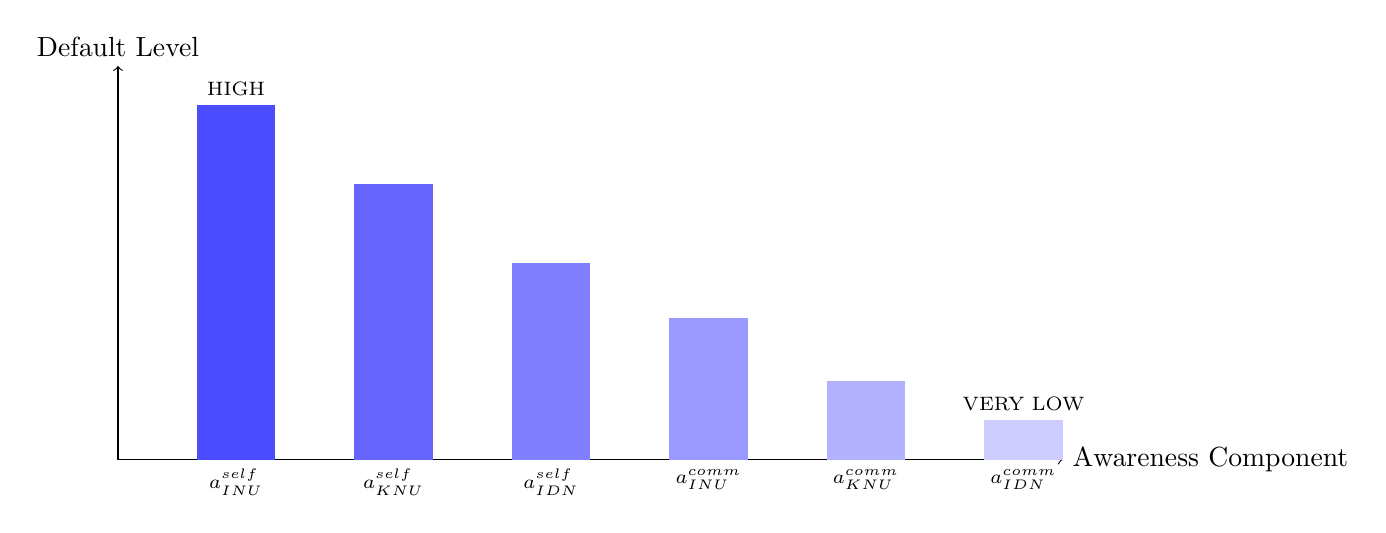
\begin{tikzpicture}
\draw[->] (0,0) -- (12,0) node[right] {Awareness Component};
\draw[->] (0,0) -- (0,5) node[above] {Default Level};

\fill[blue!70] (1,4.5) rectangle (2,0);
\fill[blue!60] (3,3.5) rectangle (4,0);
\fill[blue!50] (5,2.5) rectangle (6,0);
\fill[blue!40] (7,1.8) rectangle (8,0);
\fill[blue!30] (9,1.0) rectangle (10,0);
\fill[blue!20] (11,0.5) rectangle (12,0);

\node[below, font=\scriptsize] at (1.5,0) {$a^{self}_{INU}$};
\node[below, font=\scriptsize] at (3.5,0) {$a^{self}_{KNU}$};
\node[below, font=\scriptsize] at (5.5,0) {$a^{self}_{IDN}$};
\node[below, font=\scriptsize] at (7.5,0) {$a^{comm}_{INU}$};
\node[below, font=\scriptsize] at (9.5,0) {$a^{comm}_{KNU}$};
\node[below, font=\scriptsize] at (11.5,0) {$a^{comm}_{IDN}$};

\node[above, font=\scriptsize] at (1.5,4.5) {HIGH};
\node[above, font=\scriptsize] at (11.5,0.5) {VERY LOW};
\end{tikzpicture}
\caption{Default Awareness Gradient}
\label{fig:awareness-gradient}
\end{figure}

This gradient explains why:
\begin{itemize}
\item Self-interest dominates by default
\item Collective concerns require activation
\item Others' welfare requires deliberate perspective-taking
\item Others' identity is rarely considered
\end{itemize}

%%%%%%%%%%%%%%%%%%%%%%%%%%%%%%%%%%%%%%%%%%%%%%%%%%%%%%%%%%%%%%%%%%%%%%%%%%%%%%%
\subsection{The Effective Welfare Function with Two-Level Awareness}
\label{subsec:effective-welfare-awareness}
%%%%%%%%%%%%%%%%%%%%%%%%%%%%%%%%%%%%%%%%%%%%%%%%%%%%%%%%%%%%%%%%%%%%%%%%%%%%%%%

\subsubsection{From Full Welfare to Effective Welfare}

\paragraph{Full Welfare (from Chapter 10).}
The complete welfare function considers all effects:

\begin{equation}
Q^{full} = Q^{self} + Q^{community}
\end{equation}

where:
\begin{align}
Q^{self} &= \omega^{self}_{INU} \cdot U^{self}_{INU} + \omega^{self}_{KNU} \cdot U^{self}_{KNU} + \omega^{self}_{IDN} \cdot U^{self}_{IDN} + \text{complementarities} \\
Q^{community} &= \omega^{comm}_{INU} \cdot U^{comm}_{INU} + \omega^{comm}_{KNU} \cdot U^{comm}_{KNU} + \omega^{comm}_{IDN} \cdot U^{comm}_{IDN} + \text{complementarities}
\end{align}

\paragraph{Effective Welfare (filtered by Awareness).}
What actually guides decisions:

\begin{equation}
\boxed{
Q^{eff} = \sum_{j \in \{self, comm\}} \sum_{i \in \{INU, KNU, IDN\}} a^j_i \cdot \omega^j_i \cdot U^j_i
}
\label{eq:effective-welfare-complete}
\end{equation}

Expanded:
\begin{align}
Q^{eff} = \quad & a^{self}_{INU} \cdot \omega^{self}_{INU} \cdot U^{self}_{INU} \nonumber \\
+ \quad & a^{self}_{KNU} \cdot \omega^{self}_{KNU} \cdot U^{self}_{KNU} \nonumber \\
+ \quad & a^{self}_{IDN} \cdot \omega^{self}_{IDN} \cdot U^{self}_{IDN} \nonumber \\
+ \quad & a^{comm}_{INU} \cdot \omega^{comm}_{INU} \cdot U^{comm}_{INU} \nonumber \\
+ \quad & a^{comm}_{KNU} \cdot \omega^{comm}_{KNU} \cdot U^{comm}_{KNU} \nonumber \\
+ \quad & a^{comm}_{IDN} \cdot \omega^{comm}_{IDN} \cdot U^{comm}_{IDN}
\end{align}

\subsubsection{The Three Multiplicative Factors}

For each component, behavior is driven by \emph{three} factors:

\begin{equation}
\text{Effective contribution} = a \cdot \omega \cdot U
\end{equation}

\begin{table}[htbp]
\centering
\caption{The Three Factors Determining Behavioral Impact}
\label{tab:three-factors}
\renewcommand{\arraystretch}{1.4}
\begin{tabular}{@{}llll@{}}
\toprule
\textbf{Factor} & \textbf{Symbol} & \textbf{Question} & \textbf{Changeability} \\
\midrule
Awareness & $a$ & Am I thinking about it? & Fast (situational) \\
Weight & $\omega$ & How much do I care? & Slow (values) \\
Utility & $U$ & How large is the effect? & Via design/policy \\
\bottomrule
\end{tabular}
\end{table}

\paragraph{Implication for Intervention.}
Behavior can be changed by targeting any of the three factors:

\begin{itemize}
\item \textbf{Increase $a$:} Nudges, reminders, framing, salience
\item \textbf{Increase $\omega$:} Education, value change, identity work
\item \textbf{Increase $U$:} Incentive design, policy, environmental change
\end{itemize}

%%%%%%%%%%%%%%%%%%%%%%%%%%%%%%%%%%%%%%%%%%%%%%%%%%%%%%%%%%%%%%%%%%%%%%%%%%%%%%%
\subsection{Determinants of Awareness}
\label{subsec:awareness-determinants}
%%%%%%%%%%%%%%%%%%%%%%%%%%%%%%%%%%%%%%%%%%%%%%%%%%%%%%%%%%%%%%%%%%%%%%%%%%%%%%%

\subsubsection{What Shapes Each Awareness Component?}

\paragraph{Determinants of Own Utility Awareness ($a^{self}$).}

\begin{table}[htbp]
\centering
\caption{Determinants of Own Utility Awareness}
\label{tab:determinants-self}
\renewcommand{\arraystretch}{1.3}
\begin{tabular}{@{}llll@{}}
\toprule
\textbf{Factor} & $a^{self}_{INU}$ & $a^{self}_{KNU}$ & $a^{self}_{IDN}$ \\
\midrule
Default (no cues) & HIGH & Medium & Low \\
Time pressure & ↑↑ & ↓ & ↓ \\
``For you'' framing & ↑↑ & ↓ & ↓ \\
``For us'' framing & ↓ & ↑↑ & ↑ \\
Group presence & ↓ & ↑↑ & ↑ \\
Identity prime & ↓ & ↑ & ↑↑ \\
Value conflict & ~ & ~ & ↑↑ \\
Cognitive load & ↑ & ↓ & ↓ \\
\bottomrule
\end{tabular}
\end{table}

\paragraph{Determinants of Community Utility Awareness ($a^{comm}$).}

\begin{table}[htbp]
\centering
\caption{Determinants of Community Utility Awareness}
\label{tab:determinants-community}
\renewcommand{\arraystretch}{1.3}
\begin{tabular}{@{}llll@{}}
\toprule
\textbf{Factor} & $a^{comm}_{INU}$ & $a^{comm}_{KNU}$ & $a^{comm}_{IDN}$ \\
\midrule
Default (no cues) & LOW & Very low & Very low \\
Others present & ↑ & ↑ & ↑ \\
Empathy induction & ↑↑ & ↑ & ↑↑ \\
Perspective-taking prompt & ↑↑ & ↑↑ & ↑↑ \\
Identifiable victim & ↑↑ & ↑ & ↑ \\
Statistical victims & ↓ & ~ & ↓ \\
Moral framing & ↑ & ↑ & ↑ \\
Leadership responsibility & ↑↑ & ↑↑ & ↑↑ \\
\bottomrule
\end{tabular}
\end{table}

\subsubsection{The Empathy-Awareness Connection}

\paragraph{Empathy Activates Community Awareness.}
Empathy is the capacity to take another's perspective, which directly 
increases $a^{comm}$:

\begin{equation}
\text{Empathy} \uparrow \quad \Rightarrow \quad a^{comm}_{INU} \uparrow, \; a^{comm}_{KNU} \uparrow, \; a^{comm}_{IDN} \uparrow
\end{equation}

\paragraph{The Identifiable Victim Effect.}
A single, identifiable person activates more community awareness than 
statistical information about many:

\begin{equation}
a^{comm}(\text{``Maria, age 7''}) >> a^{comm}(\text{``1 million children''})
\end{equation}

This explains why:
\begin{itemize}
\item Personal stories drive donations more than statistics
\item Named individuals create more policy response than aggregate data
\item ``Put a face on it'' is effective communication strategy
\end{itemize}

%%%%%%%%%%%%%%%%%%%%%%%%%%%%%%%%%%%%%%%%%%%%%%%%%%%%%%%%%%%%%%%%%%%%%%%%%%%%%%%
\subsection{Application Examples}
\label{subsec:awareness-examples}
%%%%%%%%%%%%%%%%%%%%%%%%%%%%%%%%%%%%%%%%%%%%%%%%%%%%%%%%%%%%%%%%%%%%%%%%%%%%%%%

\subsubsection{Example 1: The CEO's Layoff Decision}

A CEO must decide whether to lay off 500 employees. Awareness analysis:

\begin{table}[htbp]
\centering
\caption{CEO Layoff Decision: Awareness Levels}
\label{tab:ceo-layoff}
\renewcommand{\arraystretch}{1.3}
\begin{tabular}{@{}lccp{4cm}@{}}
\toprule
\textbf{Component} & \textbf{Default $a$} & \textbf{Should Be} & \textbf{Content} \\
\midrule
$a^{self}_{INU}$ & HIGH & -- & My bonus, reputation \\
$a^{self}_{KNU}$ & Medium & -- & Company survival \\
$a^{self}_{IDN}$ & Low & Higher & Am I a good leader? \\
$a^{comm}_{INU}$ & LOW & \textbf{HIGH} & Employees' income, stress, health \\
$a^{comm}_{KNU}$ & Very low & \textbf{HIGH} & Employees' families \\
$a^{comm}_{IDN}$ & Very low & \textbf{HIGH} & Employees' professional identity \\
\bottomrule
\end{tabular}
\end{table}

\paragraph{The Awareness Gap.}
The CEO naturally has high $a^{self}$ but low $a^{comm}$. Ethical leadership
requires raising $a^{comm}$ to consider:
\begin{itemize}
\item $a^{comm}_{INU}$: ``How does this affect each employee's livelihood?''
\item $a^{comm}_{KNU}$: ``How does this affect their families?''
\item $a^{comm}_{IDN}$: ``How does this affect their sense of professional worth?''
\end{itemize}

\subsubsection{Example 2: Climate Policy Awareness}

A citizen evaluating climate policy:

\begin{table}[htbp]
\centering
\caption{Climate Policy: Awareness Analysis}
\label{tab:climate-awareness}
\renewcommand{\arraystretch}{1.3}
\begin{tabular}{@{}lcc@{}}
\toprule
\textbf{Component} & \textbf{Typical $a$} & \textbf{Content} \\
\midrule
$a^{self}_{INU}$ & HIGH & My costs (taxes, prices) \\
$a^{self}_{KNU}$ & Medium & My family's future \\
$a^{self}_{IDN}$ & Variable & Am I environmentally responsible? \\
$a^{comm}_{INU}$ & LOW & Costs to others (workers, developing world) \\
$a^{comm}_{KNU}$ & Very low & Effects on other communities \\
$a^{comm}_{IDN}$ & Very low & Effects on others' identities \\
\bottomrule
\end{tabular}
\end{table}

\paragraph{Why Climate Action Is Hard.}
The awareness gradient works against climate action:
\begin{itemize}
\item Costs are $a^{self}_{INU}$ (high awareness): immediate, personal
\item Benefits are $a^{comm}$ (low awareness): distant others, future generations
\end{itemize}

\paragraph{Effective Climate Communication.}
Must raise $a^{comm}$ through:
\begin{itemize}
\item Identifiable affected individuals (not statistics)
\item Local impacts (raise $a^{self}_{KNU}$)
\item Identity framing (``responsible citizen'')
\end{itemize}

\subsubsection{Example 3: The Coal Miner Transition (Revisited)}

The coal miner's decision to retrain:

\begin{table}[htbp]
\centering
\caption{Coal Miner Transition: Awareness of Full Effects}
\label{tab:miner-awareness}
\renewcommand{\arraystretch}{1.3}
\begin{tabular}{@{}lccl@{}}
\toprule
\textbf{Component} & \textbf{$a$} & \textbf{$U$} & \textbf{Content} \\
\midrule
$a^{self}_{INU}$ & HIGH & +\euro{20k} & Higher salary (AWARE) \\
$a^{self}_{KNU}$ & HIGH & $-0.5$ & Leaving community (AWARE) \\
$a^{self}_{IDN}$ & HIGH & $-0.8$ & ``Not a miner anymore'' (AWARE) \\
$a^{comm}_{INU}$ & Low & ? & How does my leaving affect others? \\
$a^{comm}_{KNU}$ & Low & $-$ & Community loses a member \\
$a^{comm}_{IDN}$ & Low & $-$ & Others feel ``we're dying out'' \\
\bottomrule
\end{tabular}
\end{table}

\paragraph{The Transition Awareness Profile.}
The miner is highly aware of effects on \emph{self} (all three categories) 
but less aware of effects on \emph{community}. Interestingly, this may 
actually help the transition---full awareness of $a^{comm}$ (how leaving 
affects others) might create additional guilt and resistance.

%%%%%%%%%%%%%%%%%%%%%%%%%%%%%%%%%%%%%%%%%%%%%%%%%%%%%%%%%%%%%%%%%%%%%%%%%%%%%%%
\subsection{Nudges and Interventions Through the Awareness Lens}
\label{subsec:awareness-interventions}
%%%%%%%%%%%%%%%%%%%%%%%%%%%%%%%%%%%%%%%%%%%%%%%%%%%%%%%%%%%%%%%%%%%%%%%%%%%%%%%

\subsubsection{Nudges as Awareness Manipulation}

\paragraph{What Nudges Actually Do.}
Most behavioral interventions work by changing awareness, not preferences:

\begin{equation}
\text{Nudge} \Rightarrow \Delta a \Rightarrow \Delta Q^{eff} \Rightarrow \Delta \text{Behavior}
\end{equation}

\begin{table}[htbp]
\centering
\caption{Nudges Mapped to Awareness Components}
\label{tab:nudges-awareness-map}
\renewcommand{\arraystretch}{1.3}
\begin{tabular}{@{}lll@{}}
\toprule
\textbf{Nudge} & \textbf{Awareness Target} & \textbf{Mechanism} \\
\midrule
``For your health'' & $a^{self}_{INU,P}$ ↑ & Raises physical self-awareness \\
``For your family'' & $a^{self}_{KNU}$ ↑ & Raises collective self-awareness \\
``Be the change'' & $a^{self}_{IDN}$ ↑ & Raises identity awareness \\
``Others are affected'' & $a^{comm}_{INU}$ ↑ & Raises community awareness \\
Identifiable victim & $a^{comm}_{INU}$ ↑↑ & Strong empathy activation \\
``Their community needs...'' & $a^{comm}_{KNU}$ ↑ & Community impact salience \\
Social proof & $a^{self}_{KNU}$ ↑ & ``What we do'' framing \\
\bottomrule
\end{tabular}
\end{table}

\subsubsection{Designing Awareness-Complete Interventions}

\paragraph{The Six-Component Checklist.}
For any behavioral intervention, ask:

\begin{enumerate}
\item Does it activate $a^{self}_{INU}$? (Personal benefits/costs)
\item Does it activate $a^{self}_{KNU}$? (Group implications)
\item Does it activate $a^{self}_{IDN}$? (Identity relevance)
\item Does it activate $a^{comm}_{INU}$? (Others' individual welfare)
\item Does it activate $a^{comm}_{KNU}$? (Others' group welfare)
\item Does it activate $a^{comm}_{IDN}$? (Others' identity)
\end{enumerate}

\paragraph{Most Nudges Are Incomplete.}
Typical nudges target only 1-2 components. More comprehensive 
interventions would activate all six.

\paragraph{Example: Complete Climate Message.}

\begin{quote}
``\textbf{For you:} Save \euro{200/year on energy [$a^{self}_{INU}$]. 
\textbf{For your family:} Ensure a livable world for your grandchildren [$a^{self}_{KNU}$].
\textbf{For who you are:} Be the responsible citizen you want to be [$a^{self}_{IDN}$].
\textbf{For others:} Workers in Bangladesh face flooding [$a^{comm}_{INU}$].
\textbf{For their communities:} Entire villages are displaced [$a^{comm}_{KNU}$].
\textbf{For who they are:} Farmers lose their ancestral identity [$a^{comm}_{IDN}$].''
\end{quote}

%%%%%%%%%%%%%%%%%%%%%%%%%%%%%%%%%%%%%%%%%%%%%%%%%%%%%%%%%%%%%%%%%%%%%%%%%%%%%%%
\subsection{Summary: The Complete Awareness Framework}
\label{subsec:awareness-summary}
%%%%%%%%%%%%%%%%%%%%%%%%%%%%%%%%%%%%%%%%%%%%%%%%%%%%%%%%%%%%%%%%%%%%%%%%%%%%%%%

\begin{tcolorbox}[colback=gray!5!white, colframe=gray!75!black, title=Chapter 11 Summary: Awareness]

\textbf{Definition:}
Awareness is the consciousness of the positive and negative effects on one's 
own utility level (INU, KNU, IDN) and on the utility level (INU, KNU, IDN) 
of a relevant community, that a person has at the moment of decision.

\textbf{The Two-Level, Six-Component Structure:}
$$\mathbf{A} = \begin{pmatrix}
a^{self}_{INU} & a^{self}_{KNU} & a^{self}_{IDN} \\
a^{comm}_{INU} & a^{comm}_{KNU} & a^{comm}_{IDN}
\end{pmatrix}$$

\textbf{The Awareness Gradient:}
$$a^{self}_{INU} > a^{self}_{KNU} > a^{self}_{IDN} > a^{comm}_{INU} > a^{comm}_{KNU} > a^{comm}_{IDN}$$

\textbf{Effective Welfare:}
$$Q^{eff} = \sum_{j \in \{self, comm\}} \sum_{i \in \{INU, KNU, IDN\}} a^j_i \cdot \omega^j_i \cdot U^j_i$$

\textbf{The Three Factors:}
Behavior = $f(a \cdot \omega \cdot U)$
\begin{itemize}
\item $a$: Am I thinking about it? (fast to change)
\item $\omega$: How much do I care? (slow to change)
\item $U$: How large is the effect? (designable)
\end{itemize}

\textbf{Intervention Implications:}
\begin{itemize}
\item Most nudges target only 1-2 of 6 components
\item Complete interventions address all six
\item Community awareness ($a^{comm}$) requires deliberate activation
\item Empathy and identifiable individuals raise $a^{comm}$
\end{itemize}

\textbf{Integration with EBF:}
$$\Psi \rightarrow U \rightarrow \mathbf{A} \rightarrow Q^{eff} \rightarrow WTC \rightarrow \text{Behavior}$$

\end{tcolorbox}

%%%%%%%%%%%%%%%%%%%%%%%%%%%%%%%%%%%%%%%%%%%%%%%%%%%%%%%%%%%%%%%%%%%%%%%%%%%%%%%
% END OF CHAPTER 11
%%%%%%%%%%%%%%%%%%%%%%%%%%%%%%%%%%%%%%%%%%%%%%%%%%%%%%%%%%%%%%%%%%%%%%%%%%%%%%%
